\documentclass[a4paper,12pt,reqno,superscriptaddress,nofootinbib]{article}
%\documentclass{article}
\usepackage[centertags]{amsmath}
\usepackage{amsfonts}
\usepackage{amssymb}
\usepackage{amsthm}
\usepackage{newlfont}
\usepackage{stmaryrd}
\usepackage{mathrsfs}
\usepackage{mathtools}
\usepackage{euscript}
\usepackage{graphicx}
\usepackage{enumerate}
\usepackage{color}
\usepackage[margin=1in]{geometry}


\usepackage{hyperref}
\usepackage{physics}
\usepackage{subcaption}
\usepackage{siunitx}

\graphicspath{{./reset-plots/}}


% THEOREM-LIKE ENVIRONMENTS -----------------------------------------

\theoremstyle{plain}
\newtheorem{theorem}{Theorem}[section]
\newtheorem{corollary}[theorem]{Corollary}
\newtheorem{proposition}[theorem]{Proposition}
\newtheorem{lemma}[theorem]{Lemma}
\theoremstyle{definition}
\newtheorem{definition}[theorem]{Definition}
\newtheorem{assumption}[theorem]{Assumption}
\newtheorem{condition}[theorem]{Condition}
\newtheorem{conjecture}[theorem]{Conjecture}

\theoremstyle{remark}
\newtheorem{remark}[theorem]{Remark}
\newtheorem{note}[theorem]{Note}
\newtheorem{notes}[theorem]{Notes}
\newtheorem{example}[theorem]{Example}



% \MATHOPERATOR -----------------------------------------------------

\DeclareMathOperator{\ex}{Ex} \DeclareMathOperator{\ext}{Ext}
\DeclareMathOperator{\Int}{Int} \DeclareMathOperator{\supp}{Supp}
\DeclareMathOperator{\const}{Const}
\newcommand{\re}{\Re\,}
\newcommand{\im}{\Im\,}

\newcommand{\HH}{\mathsf{H}}
\newcommand{\PP}{\mathsf{P}}
\newcommand{\RR}{\mathsf{R}}

% GREEK - 2 letters ------------------------------------------------

\let\al=\alpha %\let\be=\beta
\let\de=\delta \let\ep=\epsilon
\let\ve=\varepsilon \let\vp=\varphi \let\ga=\gamma \let\io=\iota
\let\ka=\kappa \let\la=\lambda \let\om=\omega \let\vr=\varrho
\let\si=\sigma \let\vs=\varsigma \let\th=\theta \let\vt=\vartheta
\let\ze=\zeta \let\up=\upsilon

\let\De=\Delta \let\Ga=\chi \let\La=\Lambda \let\Om=\Omega
\let\Th=\Theta \let\Up=\Upsilon

% \MATHCAL - \ca ----------------------------------------------------


\newcommand{\be}{\begin{equation}}
	\newcommand{\en}{\end{equation}}
\def\fr{\frac}
\def\th{\theta}
\def\al{\alpha}
\def\om{\omega}
\def\ka{\kappa}
\def\ii{\textrm i}
\def\ee{\textrm e}
\def\e{\textrm e}
\def\vp{\varphi}
\def\sgn{{\textrm{sgn}}}
\def\ud{\textrm{d}}
\def\bn{{\boldsymbol \nabla}}
\def\setR{\mathbb{R}}

\let\lam=\lambda
\let\si=\sigma \let\vs=\varsigma \let\th=\theta \let\vt=\vartheta
\let\ze=\zeta \let\up=\upsilon

\let\De=\Delta \let\Ga=\Gamma \let\La=\Lambda \let\Om=\Omega
\let\Th=\Theta \let\Up=\Upsilon
\let\om=\omega



\newcommand{\caA}{{\mathcal A}}
\newcommand{\caB}{{\mathcal B}}
\newcommand{\caC}{{\mathcal C}}
\newcommand{\caD}{{\mathcal D}}
\newcommand{\caE}{{\mathcal E}}
\newcommand{\caF}{{\mathcal F}}
\newcommand{\caG}{{\mathcal G}}
\newcommand{\caH}{{\mathcal H}}
\newcommand{\caI}{{\mathcal I}}
\newcommand{\caJ}{{\mathcal J}}
\newcommand{\caK}{{\mathcal K}}
\newcommand{\caL}{{\mathcal L}}
\newcommand{\caM}{{\mathcal M}}
\newcommand{\caN}{{\mathcal N}}
\newcommand{\caO}{{\mathcal O}}
\newcommand{\caP}{{\mathcal P}}
\newcommand{\caQ}{{\mathcal Q}}
\newcommand{\caR}{{\mathcal R}}
\newcommand{\caS}{{\mathcal S}}
\newcommand{\caT}{{\mathcal T}}
\newcommand{\caU}{{\mathcal U}}
\newcommand{\caV}{{\mathcal V}}
\newcommand{\caW}{{\mathcal W}}
\newcommand{\caX}{{\mathcal X}}
\newcommand{\caY}{{\mathcal Y}}
\newcommand{\caZ}{{\mathcal Z}}

\newcommand{\bR}{\mathbb{R}}

% \MATHBB - \bb -----------------------------------------------------

\newcommand{\bba}{{\mathbb a}}
\newcommand{\bbb}{{\mathbb b}}
\newcommand{\bbc}{{\mathbb c}}
\newcommand{\bbd}{{\mathbb d}}
\newcommand{\bbe}{{\mathbb e}}
\newcommand{\bbf}{{\mathbb f}}
\newcommand{\bbg}{{\mathbb g}}
\newcommand{\bbh}{{\mathbb h}}
\newcommand{\bbi}{{\mathbb i}}
\newcommand{\bbj}{{\mathbb j}}
\newcommand{\bbk}{{\mathbb k}}
\newcommand{\bbl}{{\mathbb l}}
\newcommand{\bbm}{{\mathbb m}}
\newcommand{\bbn}{{\mathbb n}}
\newcommand{\bbo}{{\mathbb o}}
\newcommand{\bbp}{{\mathbb p}}
\newcommand{\bbq}{{\mathbb q}}
\newcommand{\bbr}{{\mathbb r}}
\newcommand{\bbs}{{\mathbb s}}
\newcommand{\bbt}{{\mathbb t}}
\newcommand{\bbu}{{\mathbb u}}
\newcommand{\bbv}{{\mathbb v}}
\newcommand{\bbw}{{\mathbb w}}
\newcommand{\bbx}{{\mathbb x}}
\newcommand{\bby}{{\mathbb y}}
\newcommand{\bbz}{{\mathbb z}}

\newcommand{\bbA}{{\mathbb A}}
\newcommand{\bbB}{{\mathbb B}}
\newcommand{\bbC}{{\mathbb C}}
\newcommand{\bbD}{{\mathbb D}}
\newcommand{\bbE}{{\mathbb E}}
\newcommand{\bbF}{{\mathbb F}}
\newcommand{\bbG}{{\mathbb G}}
\newcommand{\bbH}{{\mathbb H}}
\newcommand{\bbI}{{\mathbb I}}
\newcommand{\bbJ}{{\mathbb J}}
\newcommand{\bbK}{{\mathbb K}}
\newcommand{\bbL}{{\mathbb L}}
\newcommand{\bbM}{{\mathbb M}}
\newcommand{\bbN}{{\mathbb N}}
\newcommand{\bbO}{{\mathbb O}}
\newcommand{\bbP}{{\mathbb P}}
\newcommand{\bbQ}{{\mathbb Q}}
\newcommand{\bbR}{{\mathbb R}}
\newcommand{\bbS}{{\mathbb S}}
\newcommand{\bbT}{{\mathbb T}}
\newcommand{\bbU}{{\mathbb U}}
\newcommand{\bbV}{{\mathbb V}}
\newcommand{\bbW}{{\mathbb W}}
\newcommand{\bbX}{{\mathbb X}}
\newcommand{\bbY}{{\mathbb Y}}
\newcommand{\bbZ}{{\mathbb Z}}

\newcommand{\opunit}{\text{1}\kern-0.22em\text{l}}
\newcommand{\funit}{\mathbf{1}}

% \MATHFRAK - \fr ---------------------------------------------------

\newcommand{\ong}{\backsimeq}
\newcommand{\Z}{\mathbb Z}
\newcommand{\R}{\mathbb R}
\newcommand{\CC}{\mathbb C}
%\newcommand{\de}{\text{d}}
\newcommand{\dt}{\text{d}t}
\newcommand{\dx}{\text{d}x}
\newcommand{\dV}{\text{d}V}
\newcommand{\dr}{\text{d}r}
\newcommand{\ds}{\text{d}s}
\newcommand{\BE}{\text{BE}}
\newcommand{\een}{\mathds{1}}
\newcommand{\id}{\textrm{d}}



\newcommand{\fra}{{\mathfrak a}}
\newcommand{\frb}{{\mathfrak b}}
\newcommand{\frc}{{\mathfrak c}}
\newcommand{\frd}{{\mathfrak d}}
\newcommand{\fre}{{\mathfrak e}}
\newcommand{\frf}{{\mathfrak f}}
\newcommand{\frg}{{\mathfrak g}}
\newcommand{\frh}{{\mathfrak h}}
\newcommand{\fri}{{\mathfrak i}}
\newcommand{\frj}{{\mathfrak j}}
\newcommand{\frk}{{\mathfrak k}}
\newcommand{\frl}{{\mathfrak l}}
\newcommand{\frm}{{\mathfrak m}}
\newcommand{\frn}{{\mathfrak n}}
\newcommand{\fro}{{\mathfrak o}}
\newcommand{\frp}{{\mathfrak p}}
\newcommand{\frq}{{\mathfrak q}}
\newcommand{\frr}{{\mathfrak r}}
\newcommand{\frs}{{\mathfrak s}}
\newcommand{\frt}{{\mathfrak t}}
\newcommand{\fru}{{\mathfrak u}}
\newcommand{\frv}{{\mathfrak v}}
\newcommand{\frw}{{\mathfrak w}}
\newcommand{\frx}{{\mathfrak x}}
\newcommand{\fry}{{\mathfrak y}}
\newcommand{\frz}{{\mathfrak z}}

\newcommand{\frA}{{\mathfrak A}}
\newcommand{\frB}{{\mathfrak B}}
\newcommand{\frC}{{\mathfrak C}}
\newcommand{\frD}{{\mathfrak D}}
\newcommand{\frE}{{\mathfrak E}}
\newcommand{\frF}{{\mathfrak F}}
\newcommand{\frG}{{\mathfrak G}}
\newcommand{\frH}{{\mathfrak H}}
\newcommand{\frI}{{\mathfrak I}}
\newcommand{\frJ}{{\mathfrak J}}
\newcommand{\frK}{{\mathfrak K}}
\newcommand{\frL}{{\mathfrak L}}
\newcommand{\frM}{{\mathfrak M}}
\newcommand{\frN}{{\mathfrak N}}
\newcommand{\frO}{{\mathfrak O}}
\newcommand{\frP}{{\mathfrak P}}
\newcommand{\frQ}{{\mathfrak Q}}
\newcommand{\frR}{{\mathfrak R}}
\newcommand{\frS}{{\mathfrak S}}
\newcommand{\frT}{{\mathfrak T}}
\newcommand{\frU}{{\mathfrak U}}
\newcommand{\frV}{{\mathfrak V}}
\newcommand{\frW}{{\mathfrak W}}
\newcommand{\frX}{{\mathfrak X}}
\newcommand{\frY}{{\mathfrak Y}}
\newcommand{\frZ}{{\mathfrak Z}}

% \BOLDSYMBOL - \bs -------------------------------------------------

\newcommand{\bsa}{{\boldsymbol a}}
\newcommand{\bsb}{{\boldsymbol b}}
\newcommand{\bsc}{{\boldsymbol c}}
\newcommand{\bsd}{{\boldsymbol d}}
\newcommand{\bse}{{\boldsymbol e}}
\newcommand{\bsf}{{\boldsymbol f}}
\newcommand{\bsg}{{\boldsymbol g}}
\newcommand{\bsh}{{\boldsymbol h}}
\newcommand{\bsi}{{\boldsymbol i}}
\newcommand{\bsj}{{\boldsymbol j}}
\newcommand{\bsk}{{\boldsymbol k}}
\newcommand{\bsl}{{\boldsymbol l}}
\newcommand{\bsm}{{\boldsymbol m}}
\newcommand{\bsn}{{\boldsymbol n}}
\newcommand{\bso}{{\boldsymbol o}}
\newcommand{\bsp}{{\boldsymbol p}}
\newcommand{\bsq}{{\boldsymbol q}}
\newcommand{\bsr}{{\boldsymbol r}}
\newcommand{\bss}{{\boldsymbol s}}
\newcommand{\bst}{{\boldsymbol t}}
\newcommand{\bsu}{{\boldsymbol u}}
\newcommand{\bsv}{{\boldsymbol v}}
\newcommand{\bsw}{{\boldsymbol w}}
\newcommand{\bsx}{{\boldsymbol x}}
\newcommand{\bsy}{{\boldsymbol y}}
\newcommand{\bsz}{{\boldsymbol z}}

\newcommand{\bsA}{{\boldsymbol A}}
\newcommand{\bsB}{{\boldsymbol B}}
\newcommand{\bsC}{{\boldsymbol C}}
\newcommand{\bsD}{{\boldsymbol D}}
\newcommand{\bsE}{{\boldsymbol E}}
\newcommand{\bsF}{{\boldsymbol F}}
\newcommand{\bsG}{{\boldsymbol G}}
\newcommand{\bsH}{{\boldsymbol H}}
\newcommand{\bsI}{{\boldsymbol I}}
\newcommand{\bsJ}{{\boldsymbol J}}
\newcommand{\bsK}{{\boldsymbol K}}
\newcommand{\bsL}{{\boldsymbol L}}
\newcommand{\bsM}{{\boldsymbol M}}
\newcommand{\bsN}{{\boldsymbol N}}
\newcommand{\bsO}{{\boldsymbol O}}
\newcommand{\bsP}{{\boldsymbol P}}
\newcommand{\bsQ}{{\boldsymbol Q}}
\newcommand{\bsR}{{\boldsymbol R}}
\newcommand{\bsS}{{\boldsymbol S}}
\newcommand{\bsT}{{\boldsymbol T}}
\newcommand{\bsU}{{\boldsymbol U}}
\newcommand{\bsV}{{\boldsymbol V}}
\newcommand{\bsW}{{\boldsymbol W}}
\newcommand{\bsX}{{\boldsymbol X}}
\newcommand{\bsY}{{\boldsymbol Y}}
\newcommand{\bsZ}{{\boldsymbol Z}}

\newcommand{\scS}{{\mathscr S}}
\newcommand{\scD}{{\mathscr D}}


\newcommand{\bsalpha}{{\boldsymbol \alpha}}
\newcommand{\bsbeta}{{\boldsymbol \beta}}
\newcommand{\bsgamma}{{\boldsymbol \gamma}}
\newcommand{\bsdelta}{{\boldsymbol \delta}}
\newcommand{\bsepsilon}{{\boldsymbol \epsilon}}
\newcommand{\bsmu}{{\boldsymbol \mu}}
\newcommand{\bsomega}{{\boldsymbol \omega}}

\DeclareMathAlphabet{\mathpzc}{OT1}{pzc}{m}{it}
\newcommand{\pzo}{\mathpzc{o}}
\newcommand{\pzO}{\mathpzc{O}}


% ABBREVIATION ------------------------------------------------------

\newcommand{\fig}{Fig.\;}
\newcommand{\cf}{cf.\;}
\newcommand{\eg}{e.g.\;}
\newcommand{\ie}{i.e.\;}

% MISCELLANEOUS -----------------------------------------------------

\newcommand{\un}[1]{\underline{#1}}
\newcommand{\defin}{\stackrel{\text{def}}{=}}
\newcommand{\bound}{\partial}
\newcommand{\sbound}{\hat{\partial}}
\newcommand{\rel}{\,|\,}
\newcommand{\pnt}{\rightsquigarrow}
\newcommand{\pa}{_\bullet}
\newcommand{\nb}[1]{\marginpar{\tiny {#1}}}
\newcommand{\pair}[1]{\langle{#1}\rangle}
\newcommand{\0}{^{(0)}}
\newcommand{\1}{^{(1)}}
\newcommand{\2}{^{(2)}}
\newcommand{\tot}{_{\text{TOT}}}
\newcommand{\out}{_{\text{OUT}}}
\newcommand{\con}{_{\text{con}}}
%\newcommand{\id}{\textrm{d}}
\newcommand{\can}{\text{can}}
\newcommand{\tomean}{\stackrel{1}{\to}}
\newcommand{\rev}{_{\text{REV}}}
\newcommand{\irr}{_{\text{IRR}}}

\DeclareMathOperator{\cnst}{const}
\def\Z{\mathcal Z}
\def\cL{\mathscr L}
\def\cH{\mathscr H}
\def\cA{\mathcal A}
\def\R{\mathbb R}
\def\S{\mathcal S}
\def\mbf{\mathbf }

\def\dbar{{\mathchar'26\mkern-12mu d}}

\long\def\red#1{{\color{red}#1}}
\renewcommand\div{\mathop\mathrm{div}}


% New definition of square root:
% it renames \sqrt as \oldsqrt
\let\oldsqrt\sqrt
% it defines the new \sqrt in terms of the old one
\def\sqrt{\mathpalette\DHLhksqrt}
\def\DHLhksqrt#1#2{%
	\setbox0=\hbox{$#1\oldsqrt{#2\,}$}\dimen0=\ht0
	\advance\dimen0-0.2\ht0
	\setbox2=\hbox{\vrule height\ht0 depth -\dimen0}%
	{\box0\lower0.4pt\box2}}

\let\a=\alpha %\let\be=\beta
\let\de=\delta \let\ep=\epsilon
\let\ve=\varepsilon \let\vp=\varphi \let\ga=\gamma \let\io=\iota
\let\ka=\kappa  \let\om=\omega \let\vr=\varrho
\let\si=\sigma \let\vs=\varsigma \let\th=\theta \let\vt=\vartheta
\let\ze=\zeta \let\up=\upsilon
\let\be=\beta

\let\De=\Delta \let\Ga=\Gamma \let\La=\Lambda \let\Om=\Omega
\let\Th=\Theta

% \MATHCAL - \ca ----------------------------------------------------


\DeclareMathAlphabet{\mathpzc}{OT1}{pzc}{m}{it}


% ABBREVIATION ------------------------------------------------------

\def\bea{\begin{eqnarray}}
	\def\eea{\end{eqnarray}}
\def\ba{\begin{array}}
	\def\ea{\end{array}}
\def\n{\nonumber}
\def\c{\mathscr}
\def\la{\langle}
\def\ra{\rangle}


\begin{document}
	\title{Resetting photons}	
	\author{Guilherme Eduardo Freire Oliveira, Christian Maes and Kasper Meerts\\ Instituut voor Theoretische Fysica, KU Leuven}

\begin{abstract}
Starting from a frequency diffusion process for a tagged photon which simulates relaxation to the Planck law, we introduce a resetting where photons lower their frequency at random times.
We consider two versions, one where the resetting to low frequency is independent of the existing frequency and a second case where the reduction in frequency scales with the original frequency.  The result is a nonlinear Markov process where the stationary distribution modifies the Planck law by abundance of low-frequency occupation. The physical relevance of such photon resetting processes can be found in explorations of nonequilibrium effects, e.g., via random expansions of a confined plasma or photon gas or via strongly inelastic scattering with matter.
\end{abstract}
\maketitle

\tableofcontents
\section{Introduction}
Resetting has been introduced and added to diffusion processes for a variety of reasons since its original conception, \cite{evans}.  Typically, optimizing search strategies has been the underlying motivation, but one can also imagine physical resettings.  By physical resettings we mean the result of a time-dependent potential, for which there are random moments of confinement, or the random appearance in certain locations of attractors, or the random contraction/expansion of an enclosed volume.  In the present paper, we investigate a new scenario where resetting is applied in frequency space of photons.  In that way we also explore physically motivated nonequilibrium effects on the Planck distribution.  At the same time, we give substance to resetting for nonlinear diffusions, \cite{przem}.\\

Resetting photons to a lower frequency refers to reducing the wave vector (in the reciprocal lattice), which, in real space, refers to an expansion. One physical mechanism we can imagine here is that of a confined plasma where the confinement is continually lifted at random moments. On the other hand, repeated inelastic scatterings of photons inside a cavity with the electrons in the wall can also provide a source for resetting behavior. We can picture that photons instantaneously lose their energy to electrons, which is rapidly dissipated to an external bath. 
Mathematically, the photon frequency may take various forms: we will focus on a resetting in terms of a Doppler shift where the frequency gets divided $\nu\rightarrow \nu/d$ by some number $d$ (divisor).  We will discuss other resetting procedures corresponding to different physical mechanisms, but they yield the same effects, as we will see.\\
To incorporate that resetting of photon frequency  $\nu$, we use a nonlinear Markov process for a tagged photon in a plasma where the main mechanism is Compton scattering.  (Other radiation processes are easy to add but are not considered here.)  The nonlinearity of the Markov process follows from the stimulated emission and the corresponding Fokker-Planck equation is the well-know Kompaneets equation.  The latter descibes relaxation to the Planck radiation law, $\propto \nu^2(\exp[\hbar\nu/(k_BT)]-1)^{-1}$.  Resetting of the frequency is added however on the level of the stochastic dynamics.  To avoid condensation of the photons at zero momentum, we apply a thermal push-back: when the tagged photon reaches zero frequency, it is re-distributed following the Planck law. The lattter may be due other sources of black-body radiation but is here used to conserve total photon number, creating a current in frequency space.\\

In the next Section we recall the elements of the Kompaneets process (without resetting) in the context of elastic Compton scattering with thermal electrons.  In Section \ref{res} we introduce the resetting mechanisms and their physical motivation.  The simulations are discussed in Section \ref{sim} and we obtain nonequilibrium photon distributions.  The abundance at low frequencies is not surprising, but interesting for understanding possible scenarios of breaking the Planck distribution of the cosmic microwave background.  Such (speculative) conclusions are presented in the final Section \ref{con}. 

\section{The Kompaneets process}

As reference process we consider a fluctuation dynamics which realizes the Kompaneets equation as its nonlinear Fokker-Planck equation \cite{paper2}.

\subsection{Kompaneets equation}
Relaxation towards equilibrium of a photon gas in contact with a nondegenerate, nonrelativistic electron bath in thermal equilibrium at temperature $T$ can be achieved via  Compton scattering.  For a dilute plasma, described by a semi-classical Boltzmann equation, Kompaneets thus arrived at an equation for the (average) occupation number $n(\tau,\omega)$ at frequency $\omega$ of the photon gas at time $\tau$, \cite{kompa}:
\begin{equation}\label{ke}
\omega^2\frac{\partial n}{\partial \tau}(\tau,\omega)= \frac{n_e\sigma_T 
	c}{m_e c^2}\frac{\partial }{\partial \omega}\omega^4\left\{k_B T 
\frac{\partial n}{\partial \omega}(\tau,\omega) + 
\hbar\left[1+n(\tau,\omega)\right]n(\tau,\omega)\right\}
\end{equation}
The constant $\sigma_T$ is the Thomson total cross section, and $n_e,m_e$ are  the density and mass of the electrons, respectively.
The stimulated emission or induced Compton scattering, \cite{liedahl, blandford}) is present in the  nonlinearity of the second term) in \eqref{ke}. Stationarity is achieved when $n(t,\omega)$ becomes the Bose-Einstein distribution with chemical potential $\mu$.

The Kompaneets equation yields a good understanding of the dynamical origina of cosmic microwave background and the related Sunyaev-Zeldovich effect \cite{sunyaeveffect,sunyaev}.  Excellent reviews include \cite{practical,gui,zeldovich}. Extensions and generalizations are e.g. obtained in \cite{buet, pitrou,barbosa, brown, itoh, itoh2, cooper, kohyama1, kohyama2, kohyama3,paper}.\\

To have a dimensionless Kompaneets equation we use $x= \hbar \omega/k_B T$, to rewrite \eqref{ke} as
\begin{equation}\label{ake}
x^2\frac{\partial n}{\partial t}(t,x) = \frac{\partial }{\partial x}x^4\left\{
\frac{\partial n}{\partial x}(t,x) + 
\left[1+n(t,x)\right]n(t,x)\right\}
\end{equation}
We also changed the time-variable into the dimensionless Compton optical depth
\[t = \frac{ k_B T }{m_e c^2} n_e \sigma_T c \, \tau\coloneqq \frac{ \tau_c}{\tau_C}\]
where $\tau_C$  is related to the Doppler shift
\begin{equation}\label{shift}
\left\langle\frac{1}{2\tau_c}\left(\frac{\Delta\omega}{\omega}\right)^2\right\rangle\approx \frac{ k_B T }{m_e c^2} n_e \sigma_T c= \frac{1}{\tau_C}
\end{equation} 
for the collision time-scale $\tau_c = \ell/c$ obtained from the mean free path of photons $\ell=(n_e\sigma_T)^{-1}$.\\

The Kompaneets equation \eqref{ake} can also be written for the photon density.  For photons in a box of volume $V$ with periodic boundary conditons, the spectral probability density equals
\begin{equation}\label{eq:spd}
\rho(t,x) = \frac{V}{N} \frac{1}{\pi^2} \left(\frac{k_B T}{\hbar c}\right)^3 
x^2 n(t,x)% = \frac{x^2 n(y,x)}{2\zeta(3) Z}
\end{equation}
where $N$ is the total number of photons.\\
When $n(t,x)= n_{BE}(x) = 1 / (\exp(x) - 1)$ (Bose-Einstein distribution) the photon number 
equals
\[
N_{BE} = 2 \zeta(3) \frac{V}{\pi^2} \left( \frac{k_B T}{\hbar c} \right)^3
\]
with $\zeta(3) = 1/2 \int_0^\infty \id x x^2/(e^x-1) \simeq 1.202$, and the spectral probability density is $ \rho_{BE}(x) = \frac{x^2 n_{BE}(x)}{2\zeta(3)}$.\\
Then,  in terms of the photon spectral density \eqref{eq:spd}, the Kompaneets equation \eqref{ake} becomes
\begin{equation}\label{kp}
\frac{\partial \rho}{\partial t} (t,x) = -\frac{\partial}{\partial x}\left[\left(4x- x^2\left(1+2\zeta(3) \,\frac{\rho(t,x)}{x^2}\right)\right)\rho(t,x)\right] + \frac{\partial^2}{\partial x^2}\left[x^2 \rho(t,x)\right]
\end{equation}


\subsection{Tagged photon stochastic process}
The Kompaneets equation is positivity preserving \cite{positivity}. It allows therefore a probabilistic interpretation as nonlinear Fokker-Planck equation. That was explicitly realized in \cite{fre}, and we refer to it as the Kompaneets process. \\
We constructed there the tagged photon diffusion process,
\begin{equation} \label{kp-ito2}
\dot x	= \frac{\dd {B}}{\dd x}(x) - \beta {B}(x) {U'}(x)(1+n(t,x)) +   2\frac{{B}(x)}{x} + \sqrt{2{B}(x)}\, \xi_t
\end{equation}
where $\xi_t$ is standard white noise.  Note that we need to know the particle number to use the relation \eqref{eq:spd} for finding the occupation number $n(t,x)$ from the density $\rho(t,x)$.   In our case, particle number is conserved.\\
The It\^o stochastic process \eqref{kp-ito2} is our Kompaneets process, a (nonlinear) Langevin dynamics associated to the Kompaneets equation \eqref{kp} in the case where
\[
U(x) = x,\qquad B(x) = x^2
\]  
Even without explicit boundary conditions, there is no probability flux through the origin $\nu=0$, meaning that negative frequencies are not observed. On the other hand and physically speaking, reaction processes such as Bremsstrahlung or double Compton scattering control the photon number density, picking up and absorbing photons with low-enough frequencies, but we ignore the detailed implementation of these processes in the present work.\\
  
As an illustration of the soundness of the process, we reproduce here the results obtained from the simulation of the stochastic equation \eqref{kp} using the Euler-Maruyama algorithm \cite{toral}. To implement stimulated emission, which makes a nontrivial aspect both in the simulation and theory, we consider an ensemble of $N$ processes, using the empirical histogram of frequencies to update the drift term at each timestep accordingly. The details of the implementation including reactive mechanisms together with a more comprehensive discussion can be found in \cite{paper2}. From Fig.\ref{fig:spd-kompaneets} we see relaxation towards Planck law in time, confirming the validity of the implementation scheme.
  
\begin{figure}
	\includegraphics{{spd_N-1e6.00_dx-0.05_t-3_dt-0.0001_ic-hotplanck}.pdf}
	\caption{Result of Kompaneets, for three units of time.  Needs indication of what in axes.  Mention maximum excess of 1/1000.  Mention very fastg prethermalization, slow final thermalization --- low frequency going like $x$.}
	\label{fig:spd-kompaneets}
\end{figure}

\section{Resetting Kompaneets process}\label{res}

We start from the Kompaneets process defined in the previous section and add Poissonian resetting with 
a constant rate. The resetting rate is denoted by $r$. Three methods are 
introduced for resetting, the so-called ``division'' method, where the energy of 
the photon is divided by a constant factor $d$, the ``uniform'' method, where the 
photon's energy is reset to a random value uniformly distributed between 0 and 
a cutoff $2x_0$, and finally the ``exponential'' method, where the new energy of 
the photon follows an exponential distribution with scale $x_0$.

For a justification of the mechanisms underlying this resetting we turn our 
attention towards two phenomena: the metric expansion of space and the Doppler 
effect. From the beginning of the lepton era to the time of recombination, space has 
expanded a millionfold, and from recombination until now the scale factor has 
increased by another factor of one thousand. In the highly symmetric FLRW--solution of the Einstein field equations, this scale factor has risen 
continuously and homogeneously. Moving away from this highly idealized 
solution, we can imagine more localized, abrupt increases, applying only to a 
fraction of photons.  As a photon's frequency is inversely proportional to the 
scale factor, that in effect is a stochastic division of photon 
frequencies by some large factor. The process is reminiscent of the shift in 
frequency due to the Doppler, and in fact mathematically and conceptually that is identical to that of Doppler shifts from expanding matter.\\
 In this 
regard, one can also consider a cavity with randomly, quickly receding walls.  
Any photon catching up to these walls would again undergo a downwards shift in 
frequency.

The above  implies that the position of the photon is updated by the following 
stochastic rules: in an infinitesimal interval $\dd t$ we have
\begin{align}\label{eq:resetted-ito}
x(t + \dd t) &= x(t) + D(x,t,n_t) \dd t + \sqrt{2{B}(x)}\, \xi_t \sqrt{\dd 
t}&&\text{with probability $(1-r)\dd t$}\\\nonumber
&= \begin{cases}x(t) / d &\text{``division'' method}\\
x\sim \operatorname{Uniform}(0,x_0)&\text{``uniform'' method}\\
x\sim \operatorname{Exp}(\lambda_0)&\text{``exponential'' method}\\ 
\end{cases}&&\text{with probability $r \dd t$}
\end{align}

The resetting protocol, therefore, requires the specification of two parameters: the resetting rate $r$, which controls the strength of resetting, i.e., larger $r$ produces larger population of reset photons in the stationary distribution; and the protocol parameter $\{d,x_0,\lambda_0\}$, which controls the range in frequency space where the reset photon is placed. In that sense, the protocol parameter, acts similarly to a ``cutoff''.\\
Finally, we avoid condensation of photons at zero frequency by a thermal push-back.  In other words, whenever the tagged photon reaches zero frequency, it is getting a new frequency distributed according to the Planck law.  In that way, we create a frequency current, where the resetting drives to lower frequency and the thermal push-back induces higher frequencies (when needed).  As physical realization of that thermal push-back we may imagine other sources of black-body realization that supplement the photon gas to keep the same photon number and reach a stationary (nontrivial) distribution.

To simulate these dynamics, we revisit the procedure from \cite{paper2}.  
Adding to this, at every timestep, for every particle, we perform the resetting step with a probability $r \Delta t$. The timestep $\Delta t$ is chosen such  that this product is much smaller than 1, making sure that the probability of two resets happening in the same timestep remains negligible.

\section{Simulation result and discussion}\ref{sim}

\subsection{Discussion of results}

With the average time between resets for a given photon being hundreds to thousands of times the characteristic timescale of the stochastic process, it comes to no surprise that the deviations from the Planck law are small and mostly contained around the origin. We therefore zoom in to the lower frequencies, only showing $x$ from $0$ to $0.2$ (which is about 2\% of the full frequency range)

A first thing to observe, is that the different resetting procedures yield similar qualitative behavior by tuning properly the parameters $\{d,x_0,\lambda_0\}$.  This happens whenever the average photon frequency under the resetting distribution for different resetting protocols matches. According to our definitions for the ``uniform'' and ``exponential'' methods we have the following averages after a resetting event,
\begin{align*}\langle x \rangle_{\text{Uni}} = \frac{x_0}{2} &&\text{and}&& \langle x \rangle_\text{Exp} = \frac{1}{\lambda_0}\end{align*}
while for the ``division'' protocol, we can to a high degree of accuracy assume the photon right before resetting is distributed according to the Planck distribution, which gives it an average frequency of
\[\langle x \rangle_\text{Planck} = \int_0^{\infty}\dd x\,  x\rho_\text{Planck}(x) \approx 2.701...\]
where the Planck distribution is $\rho_\text{Planck}(x) = \frac{1}{2\zeta(3)}\frac{1}{e^{x}-1}$. Then after the division'' resetting event, the expected photon frequency is
\[\langle x\rangle_{\text{Div}}=\frac{\langle x \rangle_\text{Planck}}{d} \]

If, for the same given rate, the parameters are tuned such that these first moments coincide, we expect the different resetting protocols to produce the same behavior on average whenever
\[\langle x \rangle_\text{Uni} = \langle x \rangle_\text{Exp}=\langle x\rangle_{\text{Div}} \implies \frac{x_0}{2}=\frac{1}{\lambda_0} = \frac{\langle x \rangle_\text{Planck}}{d}.\] (\textbf{K:} why is this sufficient? because thermalization is a thousand times faster than resetting for an individual photon?)
To verify this, we perform three simulations, one for each method, with a resetting rate of \num{4e-3}, and the parameters chosen such that $\langle x \rangle$ after resetting equals $0.01$. We observe excellent agreement between the simulations as seen in Fig.\ref{fig:compare}.\\

\begin{figure}
	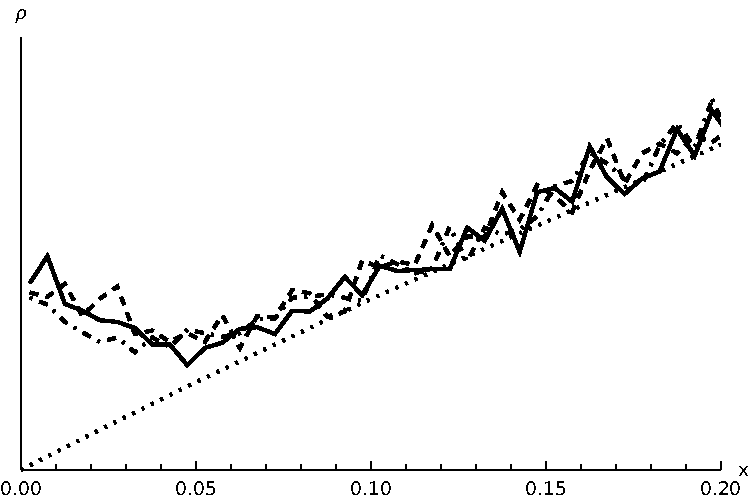
\includegraphics[width=\textwidth]{spd_compare.pdf}
	\caption{Comparison between three methods of resetting, overlaid on top of the Planck distribution (dotted straight line). All three simulations had the same resetting rate of $r=0.01$, and the resetting parameters taken to be $d=200$, $x_0\approx0.027$ and $\lambda_0\approx74$, giving approximate equal first moments of $\langle x \rangle = 0.0135...$}\label{fig:compare}
\end{figure}

That motivates  using only one resetting protocol, which is taken to be the ``division'' one. In order to explore the effects of the various parameters, we take $r=\num{2e-3}, \num{4e-3}$ and $d=160,320$. Pictures of the frequency probability distribution are showing in Fig.\ref{fig:gridplot}. We notice the presence of a non-zero amount of photons at frequency zero, rejoining the Planck distribution either gradually or with a strong jump downwards first.

\begin{figure}
	\begin{subfigure}{0.48\textwidth}
		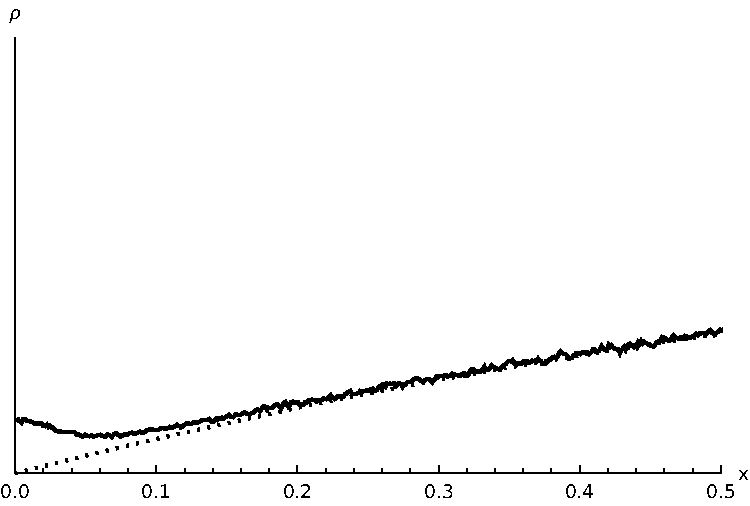
\includegraphics[width=\textwidth]{spd_r001_d100.pdf}
		\caption{$r=0.01$, $d=100$}
	\end{subfigure}\hfill
	\begin{subfigure}{0.48\textwidth}
		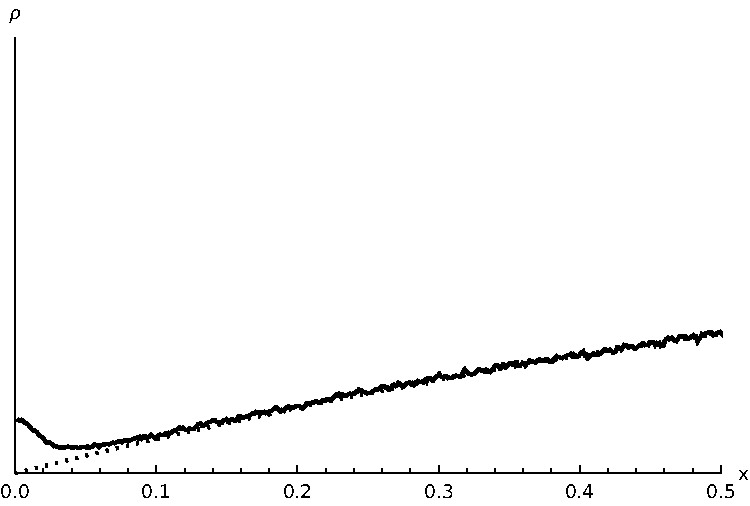
\includegraphics[width=\textwidth]{spd_r001_d200.pdf}
		\caption{$r=0.01$, $d=200$}
	\end{subfigure}
	
	\begin{subfigure}{0.48\textwidth}
		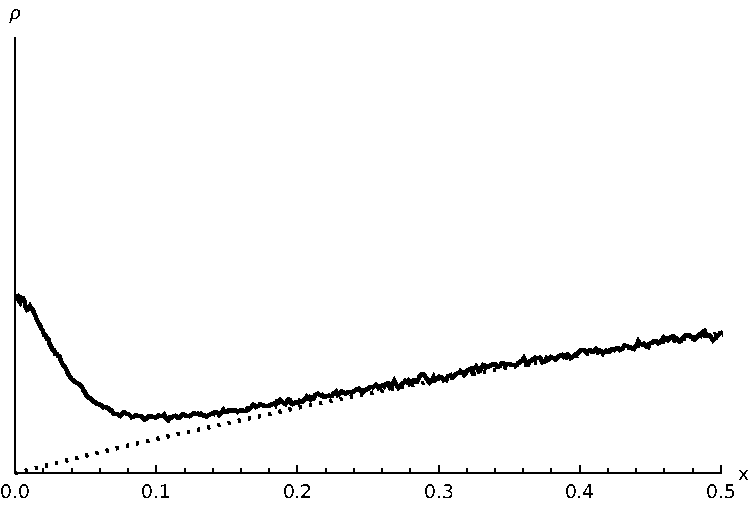
\includegraphics[width=\textwidth]{spd_r010_d100.pdf}
		\caption{$r=0.10$, $d=200$}
	\end{subfigure}\hfill
	\begin{subfigure}{0.48\textwidth}
		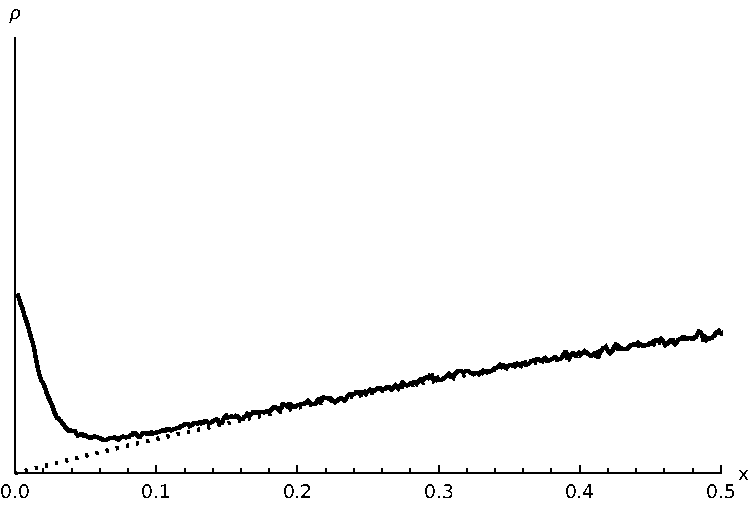
\includegraphics[width=\textwidth]{spd_r010_d200.pdf}
		\caption{$r=0.10$, $d=200$}
	\end{subfigure}

	\begin{subfigure}{0.48\textwidth}
		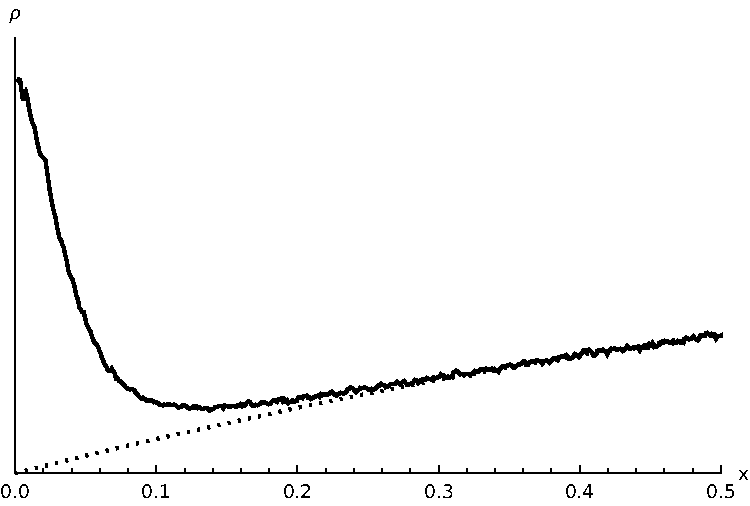
\includegraphics[width=\textwidth]{spd_r050_d100.pdf}
		\caption{$r=0.50$, $d=100$}
	\end{subfigure}\hfill
	\begin{subfigure}{0.48\textwidth}
		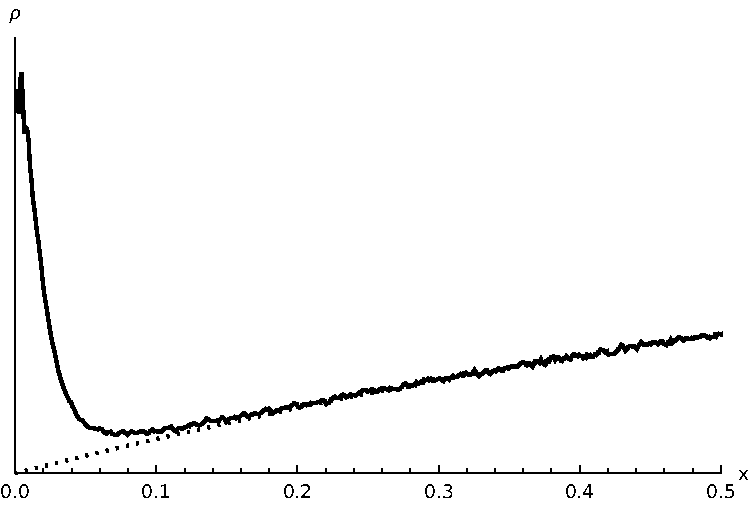
\includegraphics[width=\textwidth]{spd_r050_d200.pdf}
		\caption{$r=0.50$, $d=200$}
	\end{subfigure}
	\caption{blabla}\label{fig:gridplot}
\end{figure}

To quantify the size of the condensate near the origin, we count the number of particles with a frequency less than 0.01 (for comparison, this is 0.1\% of the support of the Planck distribution). Given the fact that our simulation consists of an ensemble of \num{1000000} particles, numerical integration of the Planck distribution tells us that in absence of resetting we can expect approximately 20 particles in this area. We plot the sizes of the condensates for various rates and divisors in figures \ref{fig:near-divisors} and \ref{fig:near-rates}. Take note that these are log-log plots. We find that for a given divisor, the relation between the number of particles near the origin and rate is close to a power-law, with an empirical exponent of about $2/3$. On the other hand, fixing the rate and varying the divisor we notice that the size of the condensate appears to rise like a power law as well (with empirical exponent $1/3$), before dropping again for higher divisors. We expect this to be a result of the high divisor bringing photons to close to zero frequency, (\textbf{K:} remark the Bremsstrahlung cross section diverges?), at which point they are very likely to be absorbed.

The expected stationary solution $\rho_Z(x)$ in the absence of resetting is also shown in the figures. We observe some general behavior: for fixed $r$, we populate lower frequencies by increasing $d$; while for fixed $d$, resetting strength is attenuated by decreasing $r$. In all those cases, deviations from the equilibrium distribution is seen only in the low-frequency regime, leading to a steady nonequilibrium state in the stationary spectral density $\rho_Z(x)$.

An important point is made by noting the formation of a condensate whenever $d$ or $r$ is increased enough. By tuning the parameters $r$ and $d$ separately, that condensate is found to be continuously formed in the $(r,d)$-plane, i.e., an abrupt transition to the condensation behavior is not found. That behavior indeed marks the appearance of a nonzero probability flux through origin, but we expect the condensate to be absorbed by including reactive mechanisms such as Bremsstrahlung or double Compton \cite{paper2}. Alternatively, reducing the $Z$ parameter as to diminish the effect of stimulated emission in the drift term appearing in \eqref{label} also prevent the condensate from forming as it is checked from the simulations.

\begin{figure}
		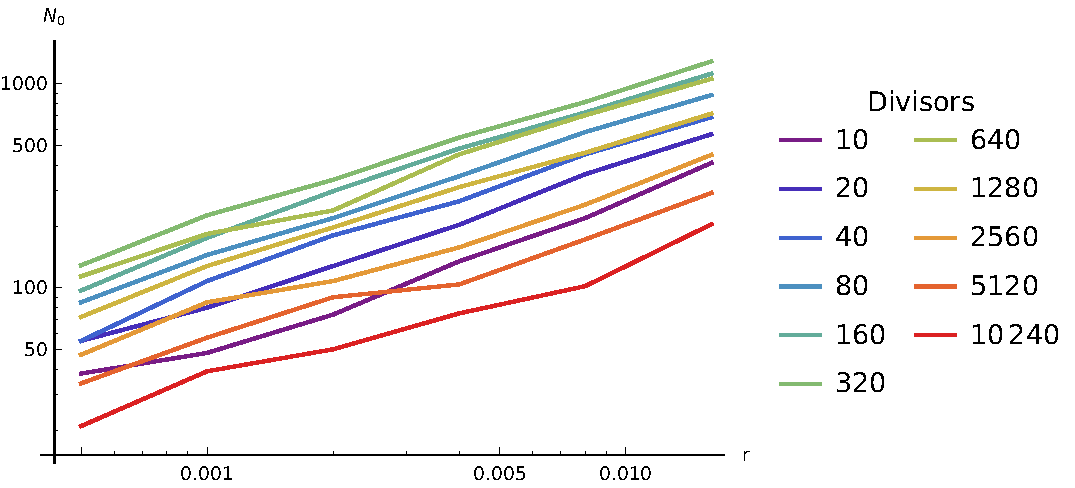
\includegraphics[width=\textwidth]{near-divisors.pdf}
		\caption{Condensate size in function of the rate for various divisors}\label{fig:near-divisors}
\end{figure}
\begin{figure}
		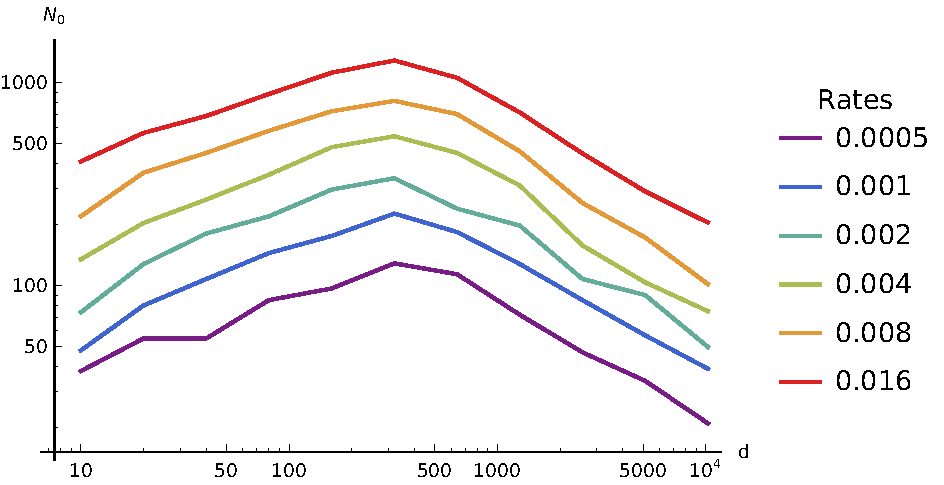
\includegraphics[width=\textwidth]{near-rates.pdf}
		\caption{Condensate size in function of the divisor for various rates}\label{fig:near-rates}
\end{figure}

The effects of resetting are negligible in the equilibrium distribution if $r$ is reduced (see Fig.\ref{label}). The threshold is found to be $r\lessapprox 10^{-3}$ for the range of parameters considered here.

\section {Conclusions}\label{con}


\bibliographystyle{abbrv}
\bibliography{langevin-kompaneets}

\end{document}
